\section{L2 Cache Size Sensitivity}
\label{sec:results:l2size_sensitivity}

In this section, we investigate how increasing the size of the private cache affects the performance of the cache partitioning algorithms.
We ran the same experiment as in section~\ref{sec:results:cache_partition}, but with varying L2 sizes.
The L2 configurations are as shown in table~\ref{tbl:processor_model:l2}, to summarize we utilize cache sizes of 128k, 256k, 512k, and 1024k.
As in previous experiments, we vary the L3 size relative to the workload size.
In this experiment, we only utilize the three random workload groups.
We do this to be able to aggregate and compare 4-core results to 8- and 16-core results.
We omit the 4-core workloads with specific traits because they would bias the overall 4-core averages.
In addition, we have only plotted STP results, this because HMS and mpki results did not add any additional insight in this experiment.

Figure~\ref{fig:results:l2:access} shows the average number of L3 accesses for random workloads with varying L2 cache size.
As can be seen from the graph, by increasing the size of the L2 cache we are decreasing the number of accesses to the L3 cache.
In other words, the L2 caches are hiding an increasing amount of memory requests from the shared level.
We expect this increased filtering of requests to have an impact on the performance of the implemented algorithms.

Figure~\ref{fig:results:l2:tadip} shows the speedup of TADIP relative to LRU measured in STP. 
As seen previously, TADIP performs as good as LRU in both 4- and 8-core workloads with a 128k L2 cache.
With increasing L2 cache size TADIP steadily outperforms LRU with between 0.1\% and 0.6\% depending on the configuration. 
At 16-cores, TADIP underperforms compared to LRU, as previously shown.
We note that, in this case, increasing the L2 size seems to cause a further decrease in TADIP performance, while the opposite is true in the 8-core case.
We expect that TADIP will react slower to changes in application phases as memory filtering increases, because of the counter architecture used to select optimal algorithms.
This effect does not seem to have a noticeable impact on results for the 4- and 8-core runs, but we assume it is causing the visible decrease in performance for the 16-core runs.

DRRIP as already covered outperforms LRU, figure~\ref{fig:results:l2:drrip} confirms this.
The figure also shows that increasing the L2 size causes a reduction in DRRIP performance.
We know that DRRIP uses a step-wise promotion policy where each successive access causes a block to be promoted by one position.
Naturally less information about success reuse will be available to the shared level as filtering in the private levels increase.
It is consequently not unexpected that DRRIP suffers from increased filtering by private cache levels.
From the figure, we note that DRRIP seems to be slightly less sensitive to small changes in L2 size with increasing core count, but in all cases a 1024k L2 causes DRRIP performance to mimic LRU performance.

In contrast to the previous algorithms, UCP performance increases with L2 cache size in all workloads, as seen in figure~\ref{fig:results:l2:ucp}.
We know that UCP uses a utility algorithm as the mechanism for allocating ways to cores. 
The input to this algorithm changes when we increase filtering of requests to the shared cache level.
As a result, the allocation of ways to cores also is expected to change, but this is the intended mechanism of UCP and should not negatively affect performance.
UCP uses LRU to manage replacement for each core, but UCP under normal circumstances only allows a core to evict one of its own blocks. 
We have already covered that this is why UCP outperforms LRU in the base configuration, in section~\ref{sec:results:cache_partition}. 
As filtering increases at the private level, we notice that UCP increases its performance compared to LRU. 
We expect that this is because, with increased private cache, more requests from recency-friendly applications can be satisfied by the private levels and less information reaches the shared level.
Trashing and streaming applications will still have its requests propagate to the shared cache, largely independent of the size of the private cache. 
Hence with increasing private cache size we expect LRU to make worse decisions by prioritizing trashing and streaming patterns due to access frequency.
UCP with utility based way-partitioning will not suffer as much from the lack of information about recency-friendly applications, and as the result show, can take advantage of increasing private cache size.

PriSM calculates target allocations for each core with the goal of reducing misses.
This technique bears some resemblance to the utility calculation done by the UMON.
As with UCP we expect PriSM to be able to increase its performance compared to LRU with increased private cache size because it will continue to limit the cache use of streaming and trashing applications.
We find this expectation reflected in our results.
For both 4- and 16-core workloads we observe an increase in performance compared to LRU as the size of private cache increases.
In the 8-core results we see the same trend between the smallest and largest L2 configuration, but we unexpectedly observe a performance drop for 256k and 512k configurations. \todo{I have no idea what is happening here...}

Finally figure~\ref{fig:results:l2:pipp} show the performance of PIPP, and figure~\ref{fig:results:l2:pipp-min8} shows the performance of the modified PIPP algorithm.
Since PIPP uses the same utility algorithm as UCP and aims to achieve the same allocations as UCP, we expect them to show similar trends.
This expectation somewhat holds true for the 4-core case, where there is a slight upward trend with increasing L2 size.
However, PIPP underperforms compared to LRU in all workloads, and with increasing core count performance drops significantly.
The expected reason behind this has already been covered in section~\ref{sec:results:cache_partition}.
The modified PIPP algorithm shows a performance development much closer to what is expected, at least for 4- and 8-core workloads.
We observe the same increase in performance with increased L2 cache size as seen in the UCP case. 
In the 16-core workloads, the performance trend is still as expected, but the modified algorithm performs worse than LRU.
This performance reduction for larger core counts has also been observed in previous research~\cite{Manikantan2012}.



\begin{figure}[!htb]
    \centering
    \begin{subfigure}[b]{0.5\textwidth}
        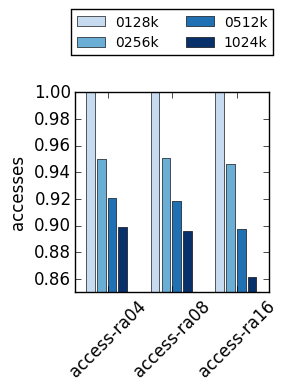
\includegraphics[width=\textwidth]{figures/results/speedup/accesses-accesses-0128k-0100-access}
        \caption{Relative number of accesses to L3 cache with varying L2 size}
        \label{fig:results:l2:access}
    \end{subfigure}
    \begin{subfigure}[b]{0.5\textwidth}
        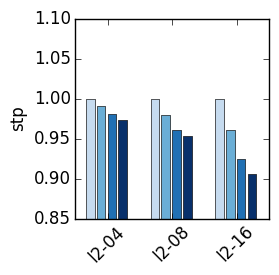
\includegraphics[width=\textwidth]{figures/results/speedup/l2-stp-0128k-tadip-l2}
        \caption{Speedup of TADIP relative to LRU}
        \label{fig:results:l2:tadip}
    \end{subfigure}%
    \begin{subfigure}[b]{0.5\textwidth}
        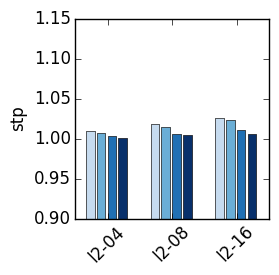
\includegraphics[width=\textwidth]{figures/results/speedup/l2-stp-0128k-drrip-3-l2}
        \caption{Speedup of DRRIP relative to LRU}
        \label{fig:results:l2:drrip}
    \end{subfigure}
\end{figure}
\clearpage
\begin{figure}[!htb]
    \ContinuedFloat
    \begin{subfigure}[b]{0.5\textwidth}
        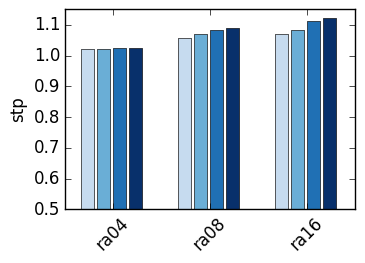
\includegraphics[width=\textwidth]{figures/results/speedup/l2-stp-0128k-ucp-l2}
        \caption{Speedup of UCP relative to LRU}
        \label{fig:results:l2:ucp}
    \end{subfigure}%
    \begin{subfigure}[b]{0.5\textwidth}
        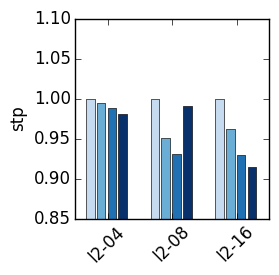
\includegraphics[width=\textwidth]{figures/results/speedup/l2-stp-0128k-prism-l2}
        \caption{Speedup of PriSM relative to LRU}
        \label{fig:results:l2:prism}
    \end{subfigure}
    \begin{subfigure}[b]{0.5\textwidth}
        \includegraphics[width=\textwidth]{figures/results/speedup/l2-stp-0128k-pipp-l2}
        \caption{Speedup of PIPP relative to LRU}
        \label{fig:results:l2:pipp}
    \end{subfigure}%
    \begin{subfigure}[b]{0.5\textwidth}
        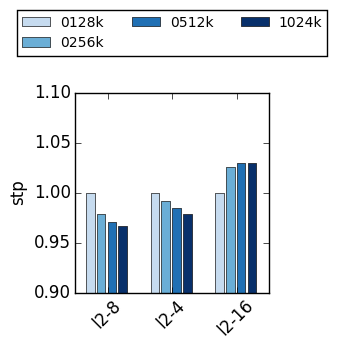
\includegraphics[width=\textwidth]{figures/results/speedup/l2-stp-0128k-pipp-min8-l2}
        \caption{Speedup of PIPP-min8 relative to LRU}
        \label{fig:results:l2:pipp-min8}
    \end{subfigure}
    \caption{Speedup of cache partition algorithms relative to LRU with increasing private L2 size}
    \label{fig:results:l2}
\end{figure}